\documentclass[aspectratio=169]{beamer}
\usetheme{Madrid}
\usepackage[utf8]{inputenc}
\usepackage[T1]{fontenc}
\usepackage{tikz}
\usepackage{amssymb}
\usepackage{graphicx}
\setbeamertemplate{navigation symbols}{}
\setbeamercolor{title}{fg=white,bg=red!75!black}
\setbeamercolor{frametitle}{fg=white,bg=red!75!black}
\setbeamercolor{block title}{bg=red!75!black!20,fg=black}
\setbeamercolor{block body}{bg=red!75!black!8,fg=black}
\setbeamercolor{item}{fg=red!75!black}
\setbeamercolor{itemize item}{fg=red!75!black}
\setbeamertemplate{itemize item}[triangle]

\title{Cyber Defense}
\subtitle{Lookalike domains, why passwords are hashed, and combining real red flags}
\author{ByteForge --- Grade 8 --- App Builder}
\date{}

\begin{document}

\begin{frame}
    \titlepage
\end{frame}

\begin{frame}{Today's Plan}
    \begin{itemize}
        \item Spot the Lookalike Domain
        \item Why Sites Never Store Your Real Password
        \item Phishing Email Red Flags
        \item[$\bigstar$] BOSS --- Build a Full Security Check
    \end{itemize}
\end{frame}

\begin{frame}{== checks EXACT equality — a lookalike is never equal}
    \large
    \begin{itemize}
        \item "rea1bank.com" (a "1" instead of "l") looks right at a glance, but \texttt{==} compares character by character
        \item Genuinely NOT equal to the real domain, even when a human skimming it would not notice.
    \end{itemize}
\end{frame}


\begin{frame}{Hashing — easy forwards, genuinely impractical backwards}
    \large
    \begin{itemize}
        \item Summing every character's ASCII code with \texttt{ord()} gives ONE number computed FROM the password
        \item But given only that number, there is no way back to which exact characters produced it.
    \end{itemize}
\end{frame}


\begin{frame}{Combining AND and OR — one function, three real signals}
    \large
    \begin{itemize}
        \item \texttt{asks\_for\_password and (urgent\_language or unknown\_sender)} makes asking for a password the non-negotiable requirement, with EITHER other signal enough to confirm it.
    \end{itemize}
\end{frame}


\begin{frame}{BOSS — layering two real functions into one decision}
    \large
    \begin{itemize}
        \item \texttt{is\_real\_domain(url) and not is\_phishing(...)}
        \item A real security system trusts multiple independent checks agreeing, never just one alone.
    \end{itemize}
\end{frame}

\begin{frame}{Real-World Examples}
    \large
    \begin{itemize}
        \item Typosquatting (registering a domain one character off from a real one) is a genuine, common real attack, not a hypothetical
        \item This chapter's exact-match check is the real defence against it. A real data breach leaking a hashed password database does not hand attackers your actual password.
    \end{itemize}
\end{frame}


\begin{frame}{Image}
    \begin{center}
    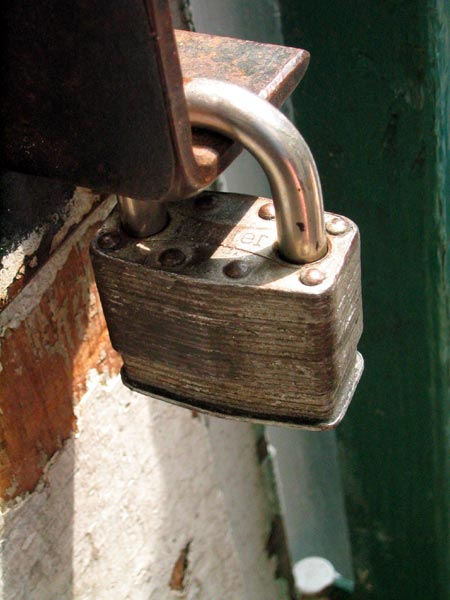
\includegraphics[width=0.5\textwidth]{images/padlock.jpg}

    \large What a hash actually protects --- easy to compute forwards, genuinely impractical to reverse.

    \small Padlock — Alyson Hurt, CC BY 2.0, via Wikimedia Commons
    \end{center}
\end{frame}

\begin{frame}{Let Them Discover}
    \Large
    Look closely at a real website address you trust. Could you spot a lookalike version of it (swapping a letter for a similar-looking number)? Try writing one out on paper.
\end{frame}

\begin{frame}{Your Turn}
    \Large
    Open the student map, find \textbf{Cyber Defense}, and work through it
    hands-on --- everything you just saw, they now do themselves.
\end{frame}

\end{document}
